%%% photextra_pipeline software paper — A&A format
\documentclass{aa}

\usepackage{graphicx}
\usepackage{txfonts}
\usepackage{natbib}
\bibpunct{(}{)}{;}{a}{}{,}
\usepackage{booktabs}
\usepackage{url}
\usepackage[colorlinks=true,linkcolor=blue,citecolor=blue,urlcolor=blue]{hyperref}
\usepackage{tikz}
\usetikzlibrary{positioning,arrows.meta,shapes.geometric,calc}

\newcommand{\photextra}{\texttt{photextra\_pipeline}}
\newcommand{\xdebpair}{\texttt{xdebpair}}
\newcommand{\xmask}{\texttt{xmask}}
\newcommand{\xpectrafit}{\texttt{XpectraFit}}
\newcommand{\arcsecond}{\ensuremath{^{\prime\prime}}}

\begin{document}

\title{PHOTometry and spectrometry EXTRAction code: multiwavelength
photo-spec pipeline to merger and no merger galaxies}

\titlerunning{\photextra: multiwavelength photo-spec pipeline for merger
and non-merger galaxies}
\authorrunning{P. Vera-Bilbao}

\author{P.~Vera-Bilbao\inst{1}}

\institute{Instituto de F\'isica y Astronom\'ia, Universidad de
Valpara\'iso, Valpara\'iso, Chile\\
\email{paulo.vb72@gmail.com}}

\date{Received --- / Accepted ---}

\abstract
% context
{Spectral energy distribution (SED) studies of galaxies in nearby clusters
increasingly require the consistent combination of multi-survey imaging
photometry with single-fibre optical spectroscopy. For interacting and
merging pairs, ground-based seeing and the broad mid-infrared point spread
functions (PSFs) blend the light of the two components, biasing both the
photometry and any derived physical parameters.}
% aims
{We present \photextra, an open-source \textsc{Python} pipeline that
automates, for arbitrary lists of targets, the retrieval of ultraviolet to
mid-infrared imaging (nine independent surveys, 21 bands) and optical
spectra, component-level deblending of close galaxy pairs,
homogenised aperture photometry, stellar+AGN spectral fitting, and a
physically motivated combination of the photometric and spectroscopic
products in a single reproducible flow.}
% methods
{From only (RA, Dec, $z$, ID) per target, the pipeline downloads GALEX,
DESI Legacy Surveys, and WISE cutouts, separates the components of close
pairs with the companion package \xdebpair, measures per-component
isolated-image photometry with PSF homogenisation to the WISE W4
resolution, resolves and fits the matching DESI or SDSS spectrum with the
companion package \xpectrafit\ (pPXF + E-MILES stellar continuum plus an
optional AGN component), and rescales the fibre spectroscopy to total
light with a wavelength-dependent aperture correction anchored on the
imaging photometry, extending the grey-factor approach of
Zou et al. (2024).}
% results
{We validate the pipeline on a controlled set of five close systems
spanning the single/companions/merger classification space, and on a
production run of 450 spectroscopic members of the galaxy cluster MKW~8
($z\simeq0.027$) from the CHANCES survey, of which 446 (99.1\,\%) yield
complete combined photometry+spectroscopy products, at a median cost of
$\simeq$220~s per target end to end and $<$1~s when resuming from cached
products.}
% conclusions
{\photextra\ provides a fully configuration-driven, checkpointable route
from target coordinates to science-ready, component-level SEDs and
aperture-corrected spectroscopic parameters, and is directly applicable to
wide-field cluster surveys such as CHANCES.}

\keywords{methods: data analysis -- techniques: photometric -- techniques:
spectroscopic -- galaxies: photometry -- galaxies: interactions --
galaxies: clusters: general}

\maketitle

%-------------------------------------------------------------------------
\section{Introduction}
\label{sec:intro}

The physical characterisation of galaxies through their spectral energy
distributions (SEDs) rests on the availability of homogeneous multi-band
photometry, and, whenever possible, on its combination with optical
spectroscopy that constrains the stellar populations, emission-line
physics and nuclear activity of the same objects
\citep[e.g.][]{boquien2019,zou2024}. Modern public surveys make the raw
ingredients abundant: the DESI Legacy Imaging Surveys \citep{dey2019}
provide deep optical $grz$ imaging over $\sim$$20\,000\,\mathrm{deg}^2$,
GALEX \citep{martin2005} and WISE \citep{wright2010} bracket the optical
with ultraviolet and mid-infrared coverage, and the DESI and SDSS
spectroscopic programmes \citep{desi2024,york2000} supply fibre spectra
for millions of galaxies. Yet assembling these ingredients into
science-ready, per-galaxy SEDs remains laborious, and three practical
problems recur.

First, \emph{resolution heterogeneity}: the PSF full width at half maximum
(FWHM) ranges from $\simeq$1.3\arcsecond\ in the Legacy Surveys optical
bands to 12\arcsecond\ in WISE W4, so consistent total-flux measurements
require PSF homogenisation, careful aperture definitions, and
per-survey zero-point handling. Second, \emph{blending}: for interacting
and merging pairs -- a population of particular interest in dense
environments -- the projected nuclear separations
($\lesssim$10\arcsecond) are comparable to or smaller than the PSF of
most of the bands involved, so the components must be deblended at the
pixel level before any per-component photometry is meaningful. Third,
\emph{aperture mismatch}: fibre spectrographs capture only the central
1.5\arcsecond\ (DESI) or 3\arcsecond\ (SDSS) of a nearby galaxy, so
spectroscopically derived quantities such as stellar masses refer to a
small and wavelength-dependent fraction of the total light and must be
tied to the imaging photometry before they can be compared with
photometric SED fits \citep{zou2024}.

General-purpose tools exist for individual steps -- source extraction
\citep{bertin1996,barbary2016}, PSF photometry, SED fitting
\citep{boquien2019}, full-spectrum fitting \citep{cappellari2017} -- but,
to our knowledge, no public pipeline chains \emph{component-level
deblending of close pairs}, \emph{multi-survey aperture photometry},
\emph{stellar+AGN spectral fitting} and a \emph{consistent
photometry--spectroscopy combination} into a single reproducible,
configuration-driven flow. \photextra\ was developed to close this gap in
the context of the CHANCES cluster survey \citep{sifon2025}, where
thousands of spectroscopic cluster members -- among them close pairs and
ongoing mergers -- must be processed uniformly.

This paper describes the design and implementation of \photextra\ and its
two scientific companion packages, \xdebpair\ (pair deblending) and
\xpectrafit\ (spectral fitting), and validates the full system on real
data. Section~\ref{sec:data} summarises the input data. Section
\ref{sec:architecture} presents the architecture and the three operation
modes. Sections~\ref{sec:photometry}--\ref{sec:combination} describe the
photometric, spectroscopic and combination stages. Section
\ref{sec:validation} reports the validation on a controlled five-system
test set and on a 450-galaxy production run on the cluster MKW~8.
Section~\ref{sec:availability} details code availability.

%-------------------------------------------------------------------------
\section{Input data}
\label{sec:data}

\subsection{Imaging}
\label{sec:data_imaging}

The pipeline supports the 21 ultraviolet-to-mid-infrared bands listed in
Table~\ref{tab:surveys}, spanning nine independent surveys, all of them
optional and selectable per run through the target configuration. Optical
$g$, $r$, $z$ cutouts are retrieved from the DESI Legacy Imaging Surveys
DR10 cutout service \citep{dey2019} at the native
$0.262\arcsecond\,\mathrm{px}^{-1}$ scale, with an exponential-backoff
retry policy against rate limiting; a bulk-download alternative for this
survey is described below. GALEX FUV/NUV and WISE W1--W4 cutouts are
retrieved through \texttt{SkyView} \citep{mcglynn1998} via
\texttt{astroquery} \citep{ginsburg2019}, requested explicitly at each
survey's native pixel scale so that the tabulated zero points apply
(Sect.~\ref{sec:calib}). SDSS $ugriz$ \citep{york2000} are likewise
retrieved through \texttt{SkyView}. Pan-STARRS1 $grizy$
\citep{chambers2016} are retrieved from the public stack-image cutout
service (\texttt{ps1images.stsci.edu}), dividing by the exposure time so
a fixed AB zero point of 25.0 applies uniformly. 2MASS $JHK_s$
\citep{skrutskie2006} are retrieved from the IRSA image-cutout service,
rescaling every per-image \texttt{MAGZP} header value to a common Vega
zero point before applying the Vega$\to$AB offset, because we found the
\texttt{SkyView} 2MASS mirror keeps the native per-image zero point,
which a single fixed value in the registry cannot represent (a
field-to-field scatter of 0.5\,mag was measured across three test
fields). Spitzer IRAC1--4 are retrieved from the public Spitzer Enhanced
Imaging Products (SEIP) mosaics via the IRSA Simple Image Access service;
because SEIP mosaics carry physical surface-brightness units
(MJy\,sr$^{-1}$) rather than raw counts, their zero point follows
directly from the pixel solid angle rather than from any catalog offset
(Table~\ref{tab:surveys}, note $c$). SEIP coverage is restricted to
targeted Spitzer fields ($\lesssim$ a few percent of the sky), so most
random sky positions legitimately return "no coverage" for this survey
alone -- a per-target coverage table and footprint map are produced by
the companion \texttt{survey\_coverage} module (Sect.~\ref{sec:coverage})
before committing to a large run.

All survey-specific properties (effective wavelength, PSF FWHM, pixel
scale, photometric zero point) are centralised in a single registry
(\texttt{SURVEY\_DEFAULTS} in \texttt{downloader.py}); no other module
hard-codes survey physics, which is what allowed the five surveys above
(SDSS, PS1, 2MASS, Spitzer, plus footprint-only support for further
archives, Sect.~\ref{sec:coverage}) to be added as a registry entry and a
retrieval function each, without touching the photometry, deblending or
spectroscopy code. The default cutout size is 1\arcmin\ (configurable),
and every downloaded image is cached on disk as FITS so that re-runs are
network-free.

\subsection{Coverage checking and non-blind bulk imaging}
\label{sec:coverage}

Two further archives are supported for \emph{coverage discovery only},
without a general-purpose per-target cutout path: the Hubble Space
Telescope archive, queried through \texttt{astroquery.mast} to report,
per target, whether any HST imaging exists nearby and in which
instrument/filter (pointed observations only, essentially never covering
a random cluster member, but occasionally relevant for special targets);
and J-PLUS, whose public SIAP footprint service answers a covered/
not-covered query without authentication even though its bulk images are
not exposed through a cutout-friendly interface. Two additional archives
with genuine imaging depth over relevant sky area -- Hyper Suprime-Cam
and S-PLUS -- were evaluated and found to require an authenticated
account for both cutouts and footprint queries; they are recorded as
\texttt{unknown (auth required)} rather than guessed. A companion module,
\texttt{survey\_coverage}, runs lightweight metadata queries (never a
full image download) for every supported archive over an arbitrary
target list and produces a per-target coverage table and a sky-position
footprint map, so that a large run can be planned -- and archives with
partial or non-existent coverage identified -- before any imaging is
retrieved.

For very large target lists ($\gtrsim10^5$), the per-target cutout
services above become rate-limit-bound rather than bandwidth-bound: at
the empirically measured $\simeq$36~s per target for the seven-band
default set, downloading cutouts for $3\times10^5$ targets one at a time
would take on the order of weeks. The pipeline therefore also supports an
opt-in bulk-download path for the Legacy Surveys imaging, the dominant
optical component: instead of one HTTP cutout request per target, the
underlying DR10 brick mosaics (fixed $0.25\times0.25\,\mathrm{deg}$
tiles tessellating the whole footprint) that actually overlap the target
list are downloaded once, in bulk, from the plain file server, and each
target's cutout is then extracted locally by WCS-based array slicing, no
further network calls involved. Because two of our target catalogues
(the CHANCES DESI cross-match and the CAVITY/Pan-STARRS-Legacy
cross-match) already carry a resolved Legacy brick identifier per
target, the set of bricks to fetch is known without any additional
spatial indexing. This conversion from $\mathcal{O}(N_\mathrm{targets})$
rate-limited requests to $\mathcal{O}(N_\mathrm{bricks})$ bulk transfers
is most valuable when targets are spatially clustered (e.g.\ cluster
members around a handful of pointings, where several targets per brick
share a single download) and provides little or no benefit when targets
are sparse across a large contiguous footprint (close to one target per
brick, so nearly the whole brick mosaic would be fetched for a single
cutout); the pipeline therefore leaves this path opt-in rather than
default, and a target list's brick-sharing ratio is the deciding factor
for whether it is worth enabling.

\begin{table}
\caption{Imaging bands supported by \photextra\ and their adopted
properties (the \texttt{SURVEY\_DEFAULTS} registry).}
\label{tab:surveys}
\centering
\begin{tabular}{lcccc}
\hline\hline
Band & $\lambda_\mathrm{eff}$ & PSF FWHM & Pixel scale & ZP$^{(a)}$ \\
     & ($\mu$m) & (\arcsecond) & (\arcsecond/px) & (AB mag) \\
\hline
GALEX FUV & 0.153 & 4.5  & 1.5   & 18.82 \\
GALEX NUV & 0.231 & 6.0  & 1.5   & 20.08 \\
SDSS $u$  & 0.355 & 1.3  & 0.396 & 22.5$^{(b)}$ \\
SDSS $g$  & 0.469 & 1.3  & 0.396 & 22.5$^{(b)}$ \\
SDSS $r$  & 0.617 & 1.3  & 0.396 & 22.5$^{(b)}$ \\
SDSS $i$  & 0.748 & 1.3  & 0.396 & 22.5$^{(b)}$ \\
SDSS $z$  & 0.893 & 1.3  & 0.396 & 22.5$^{(b)}$ \\
Legacy $g$ & 0.472 & 1.3 & 0.262 & 22.5  \\
Legacy $r$ & 0.641 & 1.3 & 0.262 & 22.5  \\
Legacy $z$ & 0.906 & 1.3 & 0.262 & 22.5  \\
PS1 $g$   & 0.487 & 1.3  & 0.25  & 25.0$^{(c)}$ \\
PS1 $r$   & 0.622 & 1.2  & 0.25  & 25.0$^{(c)}$ \\
PS1 $i$   & 0.755 & 1.1  & 0.25  & 25.0$^{(c)}$ \\
PS1 $z$   & 0.868 & 1.1  & 0.25  & 25.0$^{(c)}$ \\
PS1 $y$   & 0.963 & 1.1  & 0.25  & 25.0$^{(c)}$ \\
2MASS $J$   & 1.235 & 2.9 & 1.0  & 20.91$^{(d)}$ \\
2MASS $H$   & 1.662 & 2.9 & 1.0  & 21.39$^{(d)}$ \\
2MASS $K_s$ & 2.159 & 2.9 & 1.0  & 21.85$^{(d)}$ \\
WISE W1   & 3.4   & 6.1  & 1.375 & 23.199$^{(e)}$ \\
WISE W2   & 4.6   & 6.4  & 1.375 & 22.839$^{(e)}$ \\
WISE W3   & 12.0  & 6.5  & 1.375 & 23.174$^{(e)}$ \\
WISE W4   & 22.0  & 12.0 & 1.375 & 19.620$^{(e)}$ \\
Spitzer IRAC1 & 3.550 & 1.66 & 0.6 & 21.582$^{(f)}$ \\
Spitzer IRAC2 & 4.493 & 1.72 & 0.6 & 21.582$^{(f)}$ \\
Spitzer IRAC3 & 5.731 & 1.88 & 0.6 & 21.582$^{(f)}$ \\
Spitzer IRAC4 & 7.872 & 1.98 & 0.6 & 21.582$^{(f)}$ \\
\hline
\end{tabular}
\tablefoot{$^{(a)}$ AB zero point applying to counts on the native pixel
grid, unless noted otherwise. $^{(b)}$ SDSS is natively AB-calibrated;
small $u,z$ offsets ($\lesssim0.04$\,mag) are neglected, below the
calibration scatter. $^{(c)}$ PS1 stacks are divided by \texttt{EXPTIME}
so a fixed AB zero point of 25.0 applies (Tonry et al. 2012; Waters et
al. 2020). $^{(d)}$ 2MASS Atlas images are Vega-calibrated with a
per-image zero point (\texttt{MAGZP}); every cutout is rescaled to a
common Vega zp of 20.0 before adding the Vega$\to$AB offset (Blanton et
al. 2005: $+0.91,+1.39,+1.85$ for $J,H,K_s$). $^{(e)}$ The WISE entries
are the Atlas Vega magnitude zero points converted to AB with the
offsets of \citet{jarrett2011} ($\Delta m = 2.699, 3.339, 5.174, 6.620$
for W1--W4); see Sect.~\ref{sec:qa}. $^{(f)}$ Spitzer SEIP mosaics carry
physical units (MJy\,sr$^{-1}$); the zero point follows from the
$0.6\arcsecond$ pixel solid angle rather than from a catalog offset.}
\end{table}

\subsection{Spectroscopy}
\label{sec:data_spectra}

Targets never need to supply a spectrum file. Given (RA, Dec, $z$), the
\texttt{spectrum\_acquisition} module resolves the matching spectrum
automatically: DESI spectra are queried first through the SPARCL client
\citep{juneau2024}, with a fallback to a NOIRLab Astro Data Lab SQL query
plus direct HTTPS retrieval from the DESI DR1 healpix coadd tree when
SPARCL is unreachable; targets without a DESI match fall back to a
coordinate-based SDSS cross-match within a 3\arcsecond\ radius. Resolved
spectra are cached per target (DESI as compact \texttt{.npz} arrays of
wavelength, flux and inverse variance), so batch re-runs never re-download.
All acquisition failures are soft: a missing or unreachable spectrum can
never abort a batch run.

\subsection{Target input}

The unit of input is a target dictionary (or CSV row) with \texttt{id},
\texttt{ra}, \texttt{dec}, optional redshift \texttt{z} (required for
spectroscopy) and an optional morphological \texttt{type} column
(\texttt{merger}, \texttt{pre\_merger}, \texttt{post\_merger},
\texttt{no-merger}) that steers the separation policy
(Sect.~\ref{sec:separation_policy}). All remaining behaviour is set in a
single commented YAML configuration file; Table~\ref{tab:config}
summarises the main options.

\begin{table*}
\caption{Main configuration options of \photextra\ (YAML schema of
\texttt{config\_xmask.yaml}).}
\label{tab:config}
\centering
\begin{tabular}{llp{10.2cm}}
\hline\hline
Key & Default & Description \\
\hline
\texttt{mode} & \texttt{photometry} &
Analysis to run: \texttt{photometry}, \texttt{spectroscopy}, or
\texttt{both} (Sect.~\ref{sec:architecture}). \\
\texttt{surveys} & 9 bands &
Imaging bands to download and measure (Table~\ref{tab:surveys}). \\
\texttt{download\_size} & 1 &
Cutout width in arcmin. \\
\texttt{common\_grid.pixscale} / \texttt{.size} & 1.375 / 45 &
Common WCS grid (arcsec\,px$^{-1}$ / pixels) used for the visual
processing grid; science fluxes are measured on native pixels. \\
\texttt{use\_xdebpair} & \texttt{true} &
Use \xdebpair\ for source separation, falling back to \xmask\ and then to
a circular stub if unavailable. \\
\texttt{photometry.aperture\_mode} & \texttt{mask} &
Aperture definition: per-component pixel masks (\texttt{mask}), one fixed
circular aperture (\texttt{aperture}), or one SEP elliptical aperture
(\texttt{sep\_apertures}). \\
\texttt{photometry.separation} & \texttt{pair} &
Policy when two components are found: keep the pair (\texttt{pair},
classification-aware), measure only the central galaxy
(\texttt{central}), or one integrated measurement (\texttt{total}). \\
\texttt{photometry.aperture\_radius\_arcsec} & 5.0 &
Radius for \texttt{aperture\_mode: aperture}. \\
\texttt{sep.thresh\_sigma} / \texttt{.ellipse\_k} & 1.5 / 2.5 &
SEP detection threshold and Kron-like ellipse scale
(\texttt{sep\_apertures} mode). \\
\texttt{sep.ref\_survey} / \texttt{.max\_match\_arcsec} &
\texttt{Legacy\_r} / 10 &
Detection band and target match radius. \\
\texttt{spectroscopy.fit\_agn} & \texttt{true} &
Include an AGN component in the \xpectrafit\ fit. \\
\texttt{spectroscopy.spectrum\_fwhm} & 2.5 &
Instrumental resolution (\AA) of the spectra. \\
\texttt{spectroscopy.survey\_filters} & \texttt{[Legacy, SDSS]} &
Filter families for synthetic photometry of the spectrum. \\
\texttt{cigale\_run} / \texttt{cigale\_batch} & \texttt{false} &
Optional additional CIGALE SED fit (any mode); batch variant reuses one
model grid for all targets. \\
\texttt{output\_dir} & -- &
Root of the per-target product tree. \\
\hline
\end{tabular}
\end{table*}

%-------------------------------------------------------------------------
\section{Architecture and operation modes}
\label{sec:architecture}

\photextra\ is organised around a single orchestrator class
(\texttt{Pipeline} in \texttt{pipeline.py}) that consumes the YAML
configuration and processes one target at a time; batch drivers simply
loop (optionally in parallel) over targets. A \texttt{mode} selector
chooses among three flows (Fig.~\ref{fig:flowchart}):

\begin{itemize}
\item \texttt{photometry}: the full imaging pipeline only -- download,
  source separation, PSF homogenisation, per-component photometry, SED
  products (Sect.~\ref{sec:photometry});
\item \texttt{spectroscopy}: only spectrum acquisition and the
  \xpectrafit\ spectral fit (Sect.~\ref{sec:spectroscopy}); no imaging is
  touched;
\item \texttt{both}: the photometric pipeline plus the spectral fit, then
  the combination step that rescales the fibre spectroscopy to total
  light using the imaging photometry as absolute reference
  (Sect.~\ref{sec:combination}), producing one merged
  \texttt{\{id\}\_combined} product per target.
\end{itemize}

Each target's outputs are written under
\texttt{\{output\_dir\}/\{id\}/} in three sub-trees: \texttt{cache/}
(FITS cutouts), \texttt{products/} (machine-readable
\texttt{.csv}/\texttt{.ecsv} tables) and \texttt{plots/} (diagnostic
figures: per-band processing grids, per-component SEDs, and the combined
photometry+spectroscopy plot).

Two engineering choices proved essential for survey-scale runs. First,
\emph{checkpointing}: \texttt{Pipeline.run()} skips any target whose
final product for the selected mode already exists, and
\texttt{mode="both"} transparently reuses cached \texttt{\_photometry}
and \texttt{\_spectral} products from earlier passes, computing only the
missing pieces and the combination step -- resuming an interrupted run,
or upgrading a photometry run to a combined one, costs seconds per target
(Sect.~\ref{sec:mkw8}). Second, \emph{explicit failure accounting}: any
download or query failure is appended to a machine-readable
\texttt{failed\_targets.jsonl} manifest with a stage tag and a reason.
Critically, if the Legacy optical imaging that drives the deblending
cannot be downloaded, the pipeline refuses to degrade silently to its
built-in single-component stub mask and instead marks the target as
failed for later re-runs, so a transient rate limit can never masquerade
as a science result.

\begin{figure}
\centering
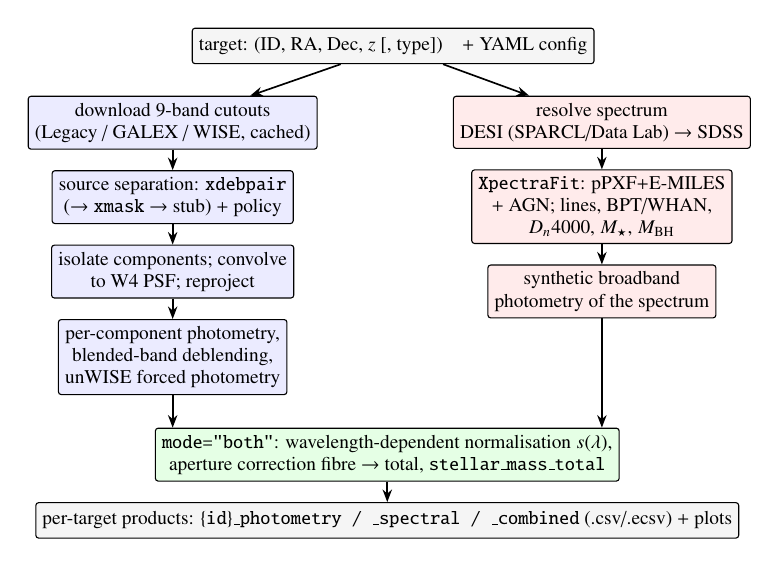
\begin{tikzpicture}[
  font=\scriptsize,
  node distance=2.6mm and 4mm,
  box/.style={draw, rounded corners=1pt, align=center,
              inner sep=2.4pt, minimum height=4.5mm, fill=gray!8},
  phot/.style={box, fill=blue!8},
  spec/.style={box, fill=red!8},
  comb/.style={box, fill=green!10},
  arr/.style={-{Stealth[length=1.6mm]}, semithick}
]
\node[box] (target) {target: (ID, RA, Dec, $z$ [, type])\quad
                      + YAML config};
\node[phot, below left=4mm and -16mm of target] (down)
  {download 9-band cutouts\\ (Legacy / GALEX / WISE, cached)};
\node[spec, below right=4mm and -18mm of target] (acq)
  {resolve spectrum\\ DESI (SPARCL/Data Lab) $\to$ SDSS};
\node[phot, below=of down] (deb)
  {source separation: \xdebpair\\ ($\to$ \xmask\ $\to$ stub) + policy};
\node[phot, below=of deb] (conv)
  {isolate components; convolve\\ to W4 PSF; reproject};
\node[phot, below=of conv] (phot)
  {per-component photometry,\\ blended-band deblending,\\
   unWISE forced photometry};
\node[spec, below=of acq] (xfit)
  {\xpectrafit: pPXF+E-MILES\\ $+$ AGN; lines, BPT/WHAN,\\
   $D_n4000$, $M_\star$, $M_\mathrm{BH}$};
\node[spec, below=of xfit] (synth)
  {synthetic broadband\\ photometry of the spectrum};
\node[comb, below=9mm of $(phot.south)!0.5!(synth.south)$] (norm)
  {\texttt{mode="both"}: wavelength-dependent normalisation
   $s(\lambda)$,\\ aperture correction fibre $\to$ total,
   \texttt{stellar\_mass\_total}};
\node[box, below=of norm] (prod)
  {per-target products: \texttt{\{id\}\_photometry / \_spectral /
   \_combined} (.csv/.ecsv) + plots};
\draw[arr] (target) -- (down);
\draw[arr] (target) -- (acq);
\draw[arr] (down) -- (deb);
\draw[arr] (deb) -- (conv);
\draw[arr] (conv) -- (phot);
\draw[arr] (acq) -- (xfit);
\draw[arr] (xfit) -- (synth);
\draw[arr] (phot.south) -- (norm.north -| phot.south);
\draw[arr] (synth.south) -- (norm.north -| synth.south);
\draw[arr] (norm) -- (prod);
\end{tikzpicture}
\caption{Architecture of \photextra. Blue boxes belong to the
\texttt{photometry} mode, red boxes to the \texttt{spectroscopy} mode;
\texttt{both} runs the two branches and the green combination step.
Every stage is checkpointed: cached products are reused and only missing
pieces are recomputed.}
\label{fig:flowchart}
\end{figure}

%-------------------------------------------------------------------------
\section{Photometric pipeline}
\label{sec:photometry}

\subsection{Source separation with \xdebpair}
\label{sec:deblending}

The default aperture definition (\texttt{aperture\_mode: mask}) assigns to
each galaxy a pixel mask per component. Masks are produced by the
companion package \xdebpair, an iterative deblending code for merging
galaxy pairs that operates on the Legacy $r$-band image (optionally with
the $g$/$z$ bands as a colour cube). \xdebpair\ first segments the field
(SEP-based segmentation, falling back to marker-controlled watershed),
identifies the nuclei, and classifies the system as \texttt{single},
\texttt{companions} (a resolved pair) or \texttt{merger} (overlapping
isophotes); for two-component systems it partitions the shared footprint
between the nuclei with a combination of watershed, two-component PSF
fitting with responsibility masks, and random-walker segmentation,
iterating to convergence on the mask intersection-over-union. The adapter
class \texttt{XdebPairAdapter} (in \texttt{deblending.py}) exposes the
result to the pipeline through a small interface (\texttt{masks},
\texttt{wcs}, \texttt{n\_components}, \texttt{separation\_arcsec},
\texttt{classification}) that is deliberately identical to that of the
simpler fallback package \xmask, so the two are interchangeable; a
built-in circular stub closes the chain for degraded environments.
Figure~\ref{fig:deblend} shows the resulting masks for the three
classification outcomes on real Legacy imaging.

\begin{figure}
\centering
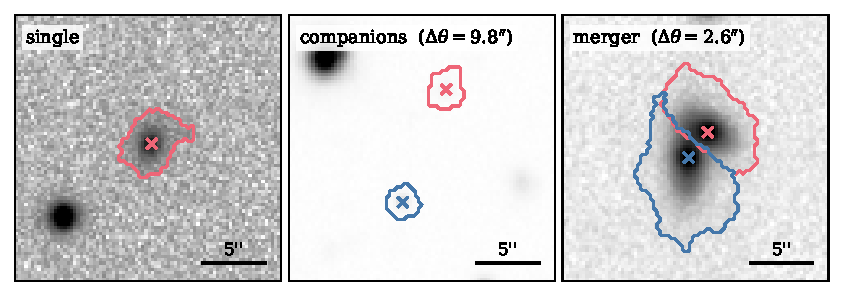
\includegraphics[width=\hsize]{figures/fig_deblend.pdf}
\caption{\xdebpair\ source separation on Legacy Survey $r$-band cutouts
for the three classification outcomes of the controlled test set
(Sect.~\ref{sec:mergers}): a single galaxy (left), a resolved pair of
companions at $\Delta\theta = 9.8\arcsecond$ (centre), and an ongoing
merger at $\Delta\theta = 2.6\arcsecond$ (right). Contours show the
per-component pixel masks (red: component 1; blue: component 2); crosses
mark the detected nuclei. Each panel is $22\arcsecond$ wide.}
\label{fig:deblend}
\end{figure}

\subsubsection{Separation policy and blending flag}
\label{sec:separation_policy}

When the target list carries a morphological \texttt{type} column, the
\texttt{photometry.separation} policy arbitrates between the
classification and the pixel-level result: with the default
\texttt{pair} policy, systems typed \texttt{merger}/\texttt{pre\_merger}
keep two components, whereas \texttt{post\_merger} or other types are
forced to a single galaxy (the union of the masks); \texttt{central}
keeps only the central component and flags the discarded companion; and
\texttt{total} always measures the mask union as one system.

Independently of the mask geometry, each band $b$ receives a per-band
blending flag,
\begin{equation}
\texttt{blend\_flag}(b) \;=\;
\bigl[\mathrm{FWHM}_\mathrm{PSF}(b) \geq \Delta\theta\bigr] ,
\label{eq:blendflag}
\end{equation}
where $\Delta\theta$ is the nuclear separation measured by \xdebpair. A
flagged band cannot resolve the pair on its own: its per-component fluxes
are reported but must be interpreted through the deblending estimators of
Sect.~\ref{sec:deblend_phot}. For the $2.6\arcsecond$ merger of
Fig.~\ref{fig:deblend}, six of the nine bands are flagged (all but the
Legacy $grz$ bands); for the $9.8\arcsecond$ companions, only WISE W4.

\subsection{PSF homogenisation and reprojection}
\label{sec:psf}

All bands are convolved to the coarsest PSF in the set (WISE W4,
12\arcsecond\ FWHM) with Gaussian matching kernels of width
$\sigma = \sqrt{\mathrm{FWHM}_\mathrm{W4}^2 - \mathrm{FWHM}_b^2}\,/\,
(2\sqrt{2\ln 2})$ per band (\texttt{convolution.py}); bands already at or
above the target resolution are left untouched (no deconvolution is
attempted). The actual pixel scale entering the kernel is always read
from each image's WCS (\texttt{\_pixscale\_from\_wcs}) rather than
trusted from the survey registry, so resampled inputs cannot silently
corrupt the kernels. Convolved images are then reprojected
(\texttt{reproject}, bilinear) onto a common TAN grid centred on the
target ($1.375\arcsecond\,\mathrm{px}^{-1}$, $45\times45$ px by default).

Two points are worth stressing. First, the full-image convolved and
reprojected frames are kept \emph{only} for the visual processing-grid
diagnostics; science fluxes are never measured on them. Second, the
per-component science measurement uses \emph{isolated} images: each
component is cut out of the native frame using its mask, individually
convolved to the common PSF and reprojected, so that the PSF wings spread
into empty sky instead of into the neighbouring component -- close-pair
flux is not cross-contaminated by the homogenisation itself
(\texttt{measure\_isolated\_photometry} in \texttt{photometry.py}).

\subsection{Flux measurement and calibration}
\label{sec:calib}

Within each mask (or aperture), background-subtracted counts are summed
and converted to flux density as
\begin{equation}
F_\nu\,[\mathrm{mJy}] = 3631\,\mathrm{Jy}\times
10^{-0.4\,\mathrm{ZP}_b}\; C_b \times 10^{3} \times
\left(p/p_0\right)^{2},
\label{eq:counts}
\end{equation}
where $C_b$ are the summed counts, $\mathrm{ZP}_b$ the AB zero point of
Table~\ref{tab:surveys}, and the last factor
(\texttt{zp\_grid\_correction}) restores the zero-point-native pixel
scale $p_0$ when the image grid has scale $p \neq p_0$: resampling
services interpolate pixel values like a surface brightness, so summed
counts scale as $(p_0/p)^2$ for a fixed sky aperture (verified
empirically by downloading the same fields at several scales). The
background level and rms are estimated from sigma-clipped statistics of
the sky pixels outside the source masks, using \texttt{sep}
\citep{barbary2016} background maps for well-sampled frames, with
coverage gaps (GALEX circular field edges, WISE tile padding) excluded.
Flux uncertainties are $\sqrt{N_\mathrm{pix}}\,\sigma_\mathrm{rms}$
converted through the same calibration.

\subsection{Deblending of blended bands and forced photometry}
\label{sec:deblend_phot}

For bands flagged by Eq.~(\ref{eq:blendflag}) the pipeline computes three
independent estimators of the flux partition between the components
(\texttt{deblend\_photometry.py}): (i) a \emph{ratio prior}, which
transports the component flux ratio measured in the unblended optical
bands to the blended band; (ii) a \emph{template fit} in the spirit of
T-PHOT-like codes, which fits the blended image with the two mask-defined
components (and optionally neighbouring sources) convolved to the band's
PSF; and (iii) a \emph{combined} estimator merging both. In addition, for
the WISE bands the pipeline queries the unWISE forced photometry of the
Legacy Surveys DR10 catalogue \citep{dey2019,lang2014}, in which the WISE
fluxes are measured by forcing the positions and morphologies of the
higher-resolution optical detections -- an external, catalogue-level
deblending that provides a valuable cross-check of the image-level
estimators. All estimators are propagated into the per-target galaxy
table so the user can compare them per band.

\subsection{Per-component SEDs}

The end product of the photometric branch is a long-format table (one row
per band) with per-component (\texttt{gal1}, \texttt{gal2}), total-system,
convolved-total and circular-aperture fluxes, blending flags and the
deblending estimators, plus per-component SED plots.
Figure~\ref{fig:seds} compares the SEDs of the three systems of
Fig.~\ref{fig:deblend}: for the resolved pair the two components are
measured independently in the unblended bands, while for the
$2.6\arcsecond$ merger the optical bands separate the components and the
encircled (blended) bands rely on the deblending estimators.

\begin{figure*}
\centering
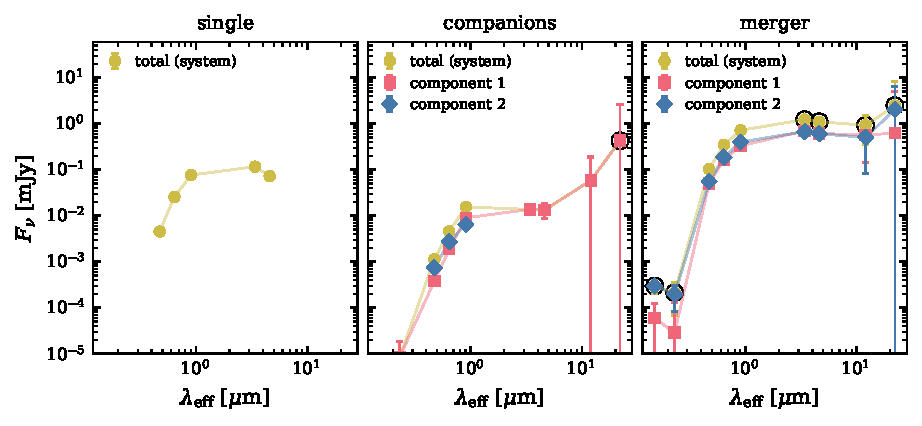
\includegraphics[width=\textwidth]{figures/fig_sed_comparison.pdf}
\caption{Per-component SEDs measured by \photextra\ for the three systems
of Fig.~\ref{fig:deblend} (from the pipeline's own photometry products).
Yellow circles: total system; red squares / blue diamonds: deblended
components. Black open circles mark bands with
$\mathrm{FWHM}_\mathrm{PSF} \geq \Delta\theta$
(Eq.~\ref{eq:blendflag}), where the per-component split relies on the
deblending estimators of Sect.~\ref{sec:deblend_phot}. Only positive
fluxes are shown.}
\label{fig:seds}
\end{figure*}

%-------------------------------------------------------------------------
\section{Spectroscopic pipeline}
\label{sec:spectroscopy}

In \texttt{spectroscopy} (and \texttt{both}) mode, the resolved spectrum
(Sect.~\ref{sec:data_spectra}) is fitted with the companion package
\xpectrafit\ through the thin adapter \texttt{run\_spectral\_fit}
(\texttt{spectral\_fit.py}). \xpectrafit's \texttt{XpectraFitter} class
orchestrates a full optical spectral analysis:

\begin{itemize}
\item \emph{Stellar continuum}: pPXF full-spectrum fitting
  \citep{cappellari2017} with the E-MILES simple stellar population
  library \citep{vazdekis2016}, yielding the stellar kinematics
  ($\sigma_\star$ and its uncertainty), mass-weighted population
  diagnostics, and fibre-aperture stellar masses;
\item \emph{AGN component}: an optional AGN continuum plus broad-line
  components (enabled by \texttt{spectroscopy.fit\_agn}), from which the
  AGN fraction \texttt{fAGN} and broad H$\alpha$/H$\beta$-based black
  hole masses $\log M_\mathrm{BH}$ are derived
  \citep[e.g.][]{greene2005};
\item \emph{Emission lines}: Gaussian measurements of 22 narrow lines
  (fluxes, equivalent widths, velocity offsets, line widths,
  signal-to-noise), feeding BPT \citep{baldwin1981,kewley2001,
  kauffmann2003} and WHAN \citep{cidfernandes2011} classifications;
\item \emph{Continuum indices}: $D_n4000$ \citep{balogh1999} and Lick
  indices;
\item \emph{Synthetic photometry}: the observed spectrum (preferred), the
  best-fit model, or the stellar continuum is integrated through the
  configured filter families (Legacy and SDSS by default), producing
  \texttt{synth\_*} broadband fluxes in the same mJy convention as the
  imaging pipeline -- the key ingredient of the combination step.
\end{itemize}

The fibre spectrum measures the \emph{total} central light of the system,
not one deblended component; the spectral products are therefore always
associated with the total aggregate, never with \texttt{gal1} or
\texttt{gal2}.

A reproducibility detail is worth recording. Early batch runs showed
run-to-run differences at the last-decimal level in some spectral
parameters: the multithreaded BLAS behind pPXF evaluates reductions in a
non-deterministic order, and a residual-to-noise ratio lying within
floating-point noise of the $\sigma$-clipping threshold could be clipped
in one run and kept in the next, occasionally toggling entire fit
branches. The fix (in \xpectrafit's \texttt{stellar.py}) rounds the
clipping ratio to eight decimals before the threshold comparison, making
the clip decision -- and thus the full pipeline -- bitwise reproducible
across runs while leaving the statistics unchanged.

%-------------------------------------------------------------------------
\section{Combining photometry and spectroscopy}
\label{sec:combination}

\subsection{Aperture normalisation}
\label{sec:norm}

In \texttt{both} mode the two branches are merged into one flat product
per target (\texttt{Pipeline.\_combine\_phot\_spec}). The physical frame
follows \citet[][Sects.~3.2--3.3]{zou2024}: the fibre spectrum suffers
aperture losses, so the imaging photometry -- which measures the whole
system -- is taken as the absolute flux reference and the spectroscopy is
corrected to total light. \citet{zou2024} apply a single grey ($r$-band)
factor; \photextra\ generalises this to a \emph{wavelength-dependent}
correction (\texttt{spec\_normalization.py}). For every configured band
whose effective wavelength lies inside the observed spectral coverage and
which has both a total-aperture imaging flux and a synthetic flux, an
anchor ratio $F_\mathrm{phot}(b)/F_\mathrm{synth}(b)$ is formed, and a
smooth scale
\begin{equation}
\ln s(\lambda) = c_0 + c_1 x + c_2 x^2, \qquad
x \equiv \ln (\lambda/\lambda_0),
\label{eq:norm}
\end{equation}
is fitted to the anchors, with $\lambda_0$ the geometric mean of the
anchor pivot wavelengths. The polynomial degree (0 = grey, 1 = colour
slope, 2 = curvature) is selected automatically and conservatively: a
degree upgrade requires enough anchors ($\geq 3$ for degree 1, $\geq 5$
for degree 2), sufficient wavelength lever arm, a BIC improvement of at
least 6, and a $\geq 5$\,\% improvement in leave-one-out cross-validation,
with 3$\sigma$ clipping of outlier anchors (at most 34\,\% clipped) and a
condition-number guard on the design matrix. With the three Legacy
anchors available today the selected degree is in practice 0 or 1; the
scheme automatically gains freedom as more bands (SDSS, HSC, S-PLUS,
J-PLUS) are added to the configuration -- the anchor collection is
generic over the survey registry, with no hard-coded band list. The
method is adapted from the normalisation introduced in the CIGALE
\texttt{cigale2s} development branch, reimplemented standalone.

Every synthetic broadband flux is rescaled by $s(\lambda)$ evaluated at
its own effective wavelength, and every emission-line flux at its own
observed wavelength, capturing differential colour/aperture mismatches a
grey factor cannot. For diagnostics, the product also carries the
historical estimators: the S/N$^2$-weighted multi-band grey factor, the
single-band ($r$) factor of \citet{zou2024}, the inter-band dispersion of
the grey ratios (values above $\sim$15--20\,\% flag strong colour
gradients or AGN contamination), and a fibre-matched recalibration
factor. The latter uses a second, always-measured set of imaging fluxes
through a synthetic aperture matched to the spectrograph fibre
(1.5\arcsecond\ DESI, 3\arcsecond\ SDSS diameter); if no total-aperture
anchor is usable the pipeline falls back to these fibre fluxes
(spectrophotometric recalibration only, flagged
\texttt{norm\_aperture="fiber\_fallback"}).

\subsection{Rescaled and invariant quantities}

Because stellar mass scales linearly with flux at fixed mass-to-light
ratio, correcting the fibre-aperture mass after the fit is equivalent to
rescaling the spectrum before it \citep{zou2024}; the product therefore
exports
\begin{equation}
M_\star^\mathrm{total} = M_\star^\mathrm{fibre}\times s(\lambda_0),
\end{equation}
(the \texttt{stellar\_mass\_total} column), keeping the original
fibre-aperture masses for diagnostics. Deliberately \emph{not} rescaled
are: the black hole masses (nonlinear in luminosity, and the unresolved
broad-line region is already fully captured by the fibre, so a
galaxy-wide aperture ratio would over-correct), the stellar velocity
dispersion, $D_n4000$, \texttt{fAGN}, and all flux-ratio classifications
(BPT/WHAN), which are aperture-independent. Figure~\ref{fig:combined}
shows the combination product for a representative cluster galaxy.

\begin{figure}
\centering
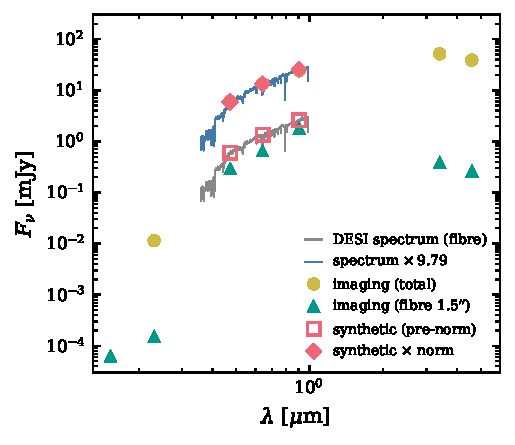
\includegraphics[width=\hsize]{figures/fig_combined_example.pdf}
\caption{Photometry--spectroscopy combination (\texttt{mode="both"}) for
a representative MKW~8 member (DESI targetid 2842593834565632,
$z=0.0279$). The observed DESI fibre spectrum (grey) under-captures the
total light measured by the imaging photometry (yellow circles) but
matches the fibre-aperture imaging fluxes (green triangles). The fitted
normalisation $s(\lambda)$ (here $\simeq 9.8$ at $\lambda_0$, anchored on
the Legacy $g$, $r$, $z$ bands) rescales the spectrum (blue) and its
synthetic photometry (open $\to$ filled red symbols) to the total-light
scale.}
\label{fig:combined}
\end{figure}

\subsection{Optional CIGALE SED fitting}

Independently of the built-in combination, the pipeline can drive CIGALE
\citep{boquien2019} as an additional SED fit in any mode
(\texttt{cigale\_integration.py}): in \texttt{both} mode with the fixed
spectroscopic redshift, broadband fluxes and the full DESI spectrum
(CIGALE's native spectrophotometric mode); in \texttt{spectroscopy} mode
on the spectrum alone; and in \texttt{photometry} mode with the redshift
left free, so CIGALE $\chi^2$-scans its redshift grid and returns a
photometric redshift (\texttt{cigale\_z\_phot}). A batch variant builds a
single multi-target input so the (expensive) model grid is computed only
once. The resulting \texttt{cigale\_*} columns (stellar mass, SFR,
$\chi^2$) are appended to the per-target products.

%-------------------------------------------------------------------------
\section{Validation}
\label{sec:validation}

\subsection{Controlled close-pair test set}
\label{sec:mergers}

The deblending-photometry chain was validated on five real systems chosen
to span the classification space (Table~\ref{tab:mergers}); three of them
are shown in Figs.~\ref{fig:deblend} and \ref{fig:seds}. The
classifications and separations are stable under re-runs, and the
per-band blending flags follow Eq.~(\ref{eq:blendflag}): the
$2.6\arcsecond$ and $4.5\arcsecond$ mergers are resolved only by the
Legacy optical bands (six of nine bands flagged), the
$9.8\arcsecond$ companion pair is blended only in WISE W4, and the single
galaxies are never flagged. In the resolved pair the independent
component SEDs recover two galaxies of comparable optical flux with
diverging mid-infrared behaviour, while in the close merger the
optical-band component split propagates consistently into the deblending
estimators of the flagged bands.

\begin{table}
\caption{Controlled five-system test set (\texttt{test\_output\_xdeb}).}
\label{tab:mergers}
\centering
\begin{tabular}{lccc}
\hline\hline
System & \xdebpair\ class & $\Delta\theta$ (\arcsecond) &
Blended bands$^{(a)}$ \\
\hline
merger\_A & merger     & 2.6 & 6/9 \\
merger\_B & companions & 9.8 & 1/9 \\
merger\_C & merger     & 4.5 & 6/9 \\
merger\_D & single     & --  & 0/9 \\
merger\_E & single     & --  & 0/9 \\
\hline
\end{tabular}
\tablefoot{$^{(a)}$ Bands with
$\mathrm{FWHM}_\mathrm{PSF}\geq\Delta\theta$ (Eq.~\ref{eq:blendflag}).}
\end{table}

\subsection{Production run: 450 members of MKW~8}
\label{sec:mkw8}

As an end-to-end test at survey scale, the pipeline was run in
\texttt{both} mode on 450 spectroscopic members of the poor cluster
MKW~8 ($z\simeq0.027$; $0.023 \leq z \leq 0.033$) from the CHANCES target
base, using seven imaging bands (GALEX FUV/NUV, Legacy $grz$, WISE
W1/W2) and automatic DESI spectrum resolution. The outcome:

\begin{itemize}
\item 446/450 targets (99.1\,\%) produced complete combined products; all
  446 spectra were resolved from DESI (SPARCL) and all 446 spectral fits
  converged (\texttt{spec\_status = ok});
\item the 4 failures were all external and transient (unWISE forced
  photometry queries exhausting their retries against a rate-limited
  VizieR mirror); they are recorded in \texttt{failed\_targets.jsonl}
  and recoverable by re-running, at which point the checkpointing
  reuses everything already computed;
\item the median end-to-end cost was $\simeq$221~s per target
  (interquartile range 181--255~s, dominated by the pPXF+AGN spectral
  fit and the image downloads), while re-entering the run with cached
  photometric and spectral products costs a median of 0.6~s per target
  for the combination step alone;
\item the total-aperture normalisation succeeded for all 446 galaxies
  (\texttt{norm\_aperture = total}, three Legacy anchors each), with a
  median aperture correction $s(\lambda_0) = 6.4$
  (16th--84th percentiles: 3.3--14.1) -- consistent with a
  1.5\arcsecond\ DESI fibre sampling the core of $z\simeq0.027$
  galaxies -- and a median inter-band ratio dispersion of 11\,\%.
\end{itemize}

Figure~\ref{fig:mkw8} summarises the distribution of aperture corrections
and the WHAN classification mix of the sample (126 star-forming, 72 sAGN,
31 wAGN, 100 retired, 35 passive, 82 unclassifiable), with the BPT
diagram yielding a consistent picture (109 SF, 73 composite, 53 LINER,
47 Seyfert); a red-sequence-dominated population with a substantial
retired/passive fraction, as expected for cluster members with a median
$D_n4000$ of 1.65.

\begin{figure*}
\centering
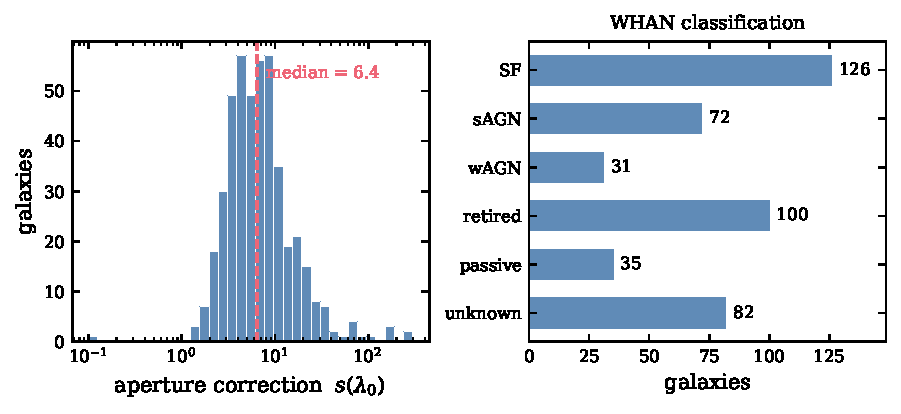
\includegraphics[width=0.86\textwidth]{figures/fig_mkw8_stats.pdf}
\caption{MKW~8 production run (446 combined products). Left: distribution
of the applied aperture correction $s(\lambda_0)$ (fibre to total light;
median 6.4, dashed line). Right: WHAN emission-line classification of the
sample as measured by \xpectrafit.}
\label{fig:mkw8}
\end{figure*}

\subsection{Quality assurance: the WISE zero-point case}
\label{sec:qa}

We report one calibration bug found and fixed during development because
it illustrates the value of physically motivated validation at the
pipeline level. The flux conversion of Eq.~(\ref{eq:counts}) assumes AB
zero points uniformly, but the WISE Atlas zero points originally entered
in the survey registry were the native \emph{Vega} magnitude zero points.
The resulting W1/W2 fluxes were inflated by roughly an order of magnitude
-- the $10^{0.4\Delta m}$ of the Vega$\to$AB offsets, a factor
$\simeq$12 in W1 and $\simeq$22 in W2. The error was caught not by unit
tests but by a physical sanity check: for normal stellar photospheres,
$F_\nu$ must decline from the 1.6\,$\mu$m stellar bump into the
mid-infrared (the Rayleigh--Jeans tail), whereas the measured
WISE-to-optical flux ratios of ordinary early-type cluster members sat an
order of magnitude above that expectation. The fix converts the WISE zero
points to AB equivalents once, in the registry, using the offsets of
\citet{jarrett2011} (Table~\ref{tab:surveys}), so the single AB
conversion of Eq.~(\ref{eq:counts}) applies uniformly to all bands. The
episode motivated the permanent inclusion of SED-level ratio diagnostics
in the validation plots, and -- together with the deterministic
$\sigma$-clipping fix of Sect.~\ref{sec:spectroscopy} and the
refuse-to-degrade download policy of Sect.~\ref{sec:architecture} --
reflects the pipeline's general design stance: failures and calibration
errors must be loud, recorded and physically checkable, never silent.

%-------------------------------------------------------------------------
\section{Code availability}
\label{sec:availability}

\photextra\ is written in \textsc{Python} ($\geq$3.8) and depends only on
standard open-source infrastructure: \texttt{numpy}, \texttt{scipy},
\texttt{astropy} \citep{astropy2022}, \texttt{matplotlib},
\texttt{photutils}, \texttt{sep} \citep{barbary2016},
\texttt{reproject}, \texttt{astroquery} \citep{ginsburg2019} and
\texttt{pyyaml}; the spectral branch additionally requires
\texttt{ppxf} \citep{cappellari2017} and the SPARCL client
\citep{juneau2024}, and the optional SED fitting requires CIGALE
\citep{boquien2019}. The package installs with \texttt{pip} and exposes
both a \textsc{Python} API (\texttt{Pipeline}) and a command-line entry
point (\texttt{photextra}) driven entirely by the YAML configuration of
Table~\ref{tab:config}. The source code of \photextra\ and of the
companion packages \xdebpair, \xmask\ and \xpectrafit\ will be released
on GitHub with an archived version on Zenodo upon publication [repository
URL, DOI and license to be finalised; license placeholder: MIT]. The
per-target products used in Sect.~\ref{sec:validation} are available from
the author on request.

%-------------------------------------------------------------------------
\section{Summary}
\label{sec:summary}

\photextra\ turns a target list of (ID, RA, Dec, $z$) into
component-level, PSF-homogenised, nine-band SEDs and aperture-corrected
spectroscopic parameters through a single configuration-driven,
checkpointed pipeline. Its distinguishing features are (i) pixel-level
deblending of close and merging pairs (\xdebpair) propagated consistently
through PSF homogenisation via isolated-component photometry and through
per-band blending flags; (ii) automatic spectrum resolution (DESI/SDSS)
and a full stellar+AGN spectral analysis (\xpectrafit); (iii) a
wavelength-dependent, conservatively regularised normalisation of the
fibre spectroscopy to total light, extending the grey aperture correction
of \citet{zou2024}; and (iv) survey-scale robustness demonstrated on 450
cluster members with a 99.1\,\% success rate and second-scale resume
cost. The pipeline is being applied to the CHANCES cluster survey and is
designed to absorb additional imaging surveys by configuration alone.

\begin{acknowledgements}
The author thanks the CHANCES collaboration. This work made use of data
from the DESI Legacy Imaging Surveys, GALEX, WISE, SDSS and DESI, and of
the NOIRLab Astro Data Lab and SPARCL services.
\end{acknowledgements}

%-------------------------------------------------------------------------
\begin{thebibliography}{}

\bibitem[Astropy Collaboration et al.(2022)]{astropy2022}
Astropy Collaboration, Price-Whelan, A.~M., Lim, P.~L., et al. 2022,
ApJ, 935, 167

\bibitem[Baldwin et al.(1981)]{baldwin1981}
Baldwin, J.~A., Phillips, M.~M., \& Terlevich, R. 1981, PASP, 93, 5

\bibitem[Balogh et al.(1999)]{balogh1999}
Balogh, M.~L., Morris, S.~L., Yee, H.~K.~C., Carlberg, R.~G., \&
Ellingson, E. 1999, ApJ, 527, 54

\bibitem[Barbary(2016)]{barbary2016}
Barbary, K. 2016, Journal of Open Source Software, 1, 58

\bibitem[Bertin \& Arnouts(1996)]{bertin1996}
Bertin, E. \& Arnouts, S. 1996, A\&AS, 117, 393

\bibitem[Boquien et al.(2019)]{boquien2019}
Boquien, M., Burgarella, D., Roehlly, Y., et al. 2019, A\&A, 622, A103

\bibitem[Cappellari(2017)]{cappellari2017}
Cappellari, M. 2017, MNRAS, 466, 798

\bibitem[Chambers et al.(2016)]{chambers2016}
Chambers, K.~C., Magnier, E.~A., Metcalfe, N., et al. 2016, arXiv:1612.05560

\bibitem[Cid Fernandes et al.(2011)]{cidfernandes2011}
Cid Fernandes, R., Stasi\'nska, G., Mateus, A., \& Vale Asari, N. 2011,
MNRAS, 413, 1687

\bibitem[DESI Collaboration et al.(2024)]{desi2024}
DESI Collaboration, Adame, A.~G., Aguilar, J., et al. 2024, AJ, 168, 58

\bibitem[Dey et al.(2019)]{dey2019}
Dey, A., Schlegel, D.~J., Lang, D., et al. 2019, AJ, 157, 168

\bibitem[Ginsburg et al.(2019)]{ginsburg2019}
Ginsburg, A., Sip\H{o}cz, B.~M., Brasseur, C.~E., et al. 2019, AJ, 157, 98

\bibitem[Greene \& Ho(2005)]{greene2005}
Greene, J.~E. \& Ho, L.~C. 2005, ApJ, 630, 122

\bibitem[Jarrett et al.(2011)]{jarrett2011}
Jarrett, T.~H., Cohen, M., Masci, F., et al. 2011, ApJ, 735, 112

\bibitem[Juneau et al.(2024)]{juneau2024}
Juneau, S., Olsen, K.~P., Nikutta, R., et al. 2024, AJ, 167, 258

\bibitem[Kauffmann et al.(2003)]{kauffmann2003}
Kauffmann, G., Heckman, T.~M., Tremonti, C., et al. 2003, MNRAS, 346, 1055

\bibitem[Kewley et al.(2001)]{kewley2001}
Kewley, L.~J., Dopita, M.~A., Sutherland, R.~S., Heisler, C.~A., \&
Trevena, J. 2001, ApJ, 556, 121

\bibitem[Lang(2014)]{lang2014}
Lang, D. 2014, AJ, 147, 108

\bibitem[Martin et al.(2005)]{martin2005}
Martin, D.~C., Fanson, J., Schiminovich, D., et al. 2005, ApJ, 619, L1

\bibitem[McGlynn et al.(1998)]{mcglynn1998}
McGlynn, T., Scollick, K., \& White, N. 1998, in IAU Symp. 179, New
Horizons from Multi-Wavelength Sky Surveys, ed. B.~J. McLean et al.
(Dordrecht: Kluwer), 465

\bibitem[Skrutskie et al.(2006)]{skrutskie2006}
Skrutskie, M.~F., Cutri, R.~M., Stiening, R., et al. 2006, AJ, 131, 1163

\bibitem[Sif\'on et al.(2025)]{sifon2025}
Sif\'on, C., et al. 2025, A\&A, in press (CHANCES survey description)

\bibitem[Vazdekis et al.(2016)]{vazdekis2016}
Vazdekis, A., Koleva, M., Ricciardelli, E., R\"ock, B., \&
Falc\'on-Barroso, J. 2016, MNRAS, 463, 3409

\bibitem[Wright et al.(2010)]{wright2010}
Wright, E.~L., Eisenhardt, P.~R.~M., Mainzer, A.~K., et al. 2010, AJ,
140, 1868

\bibitem[York et al.(2000)]{york2000}
York, D.~G., Adelman, J., Anderson, J.~E., et al. 2000, AJ, 120, 1579

\bibitem[Zou et al.(2024)]{zou2024}
Zou, F., Brandt, W.~N., Ni, Q., et al. 2024, ApJ, 961, 173

\end{thebibliography}

\end{document}
